% !TEX TS-program = lualatex
% !TEX encoding = UTF-8 Unicode
% !TEX spellcheck = de_DE
% © 2017-2023 Moritz Brinkmann, CC-by-sa
% https://ma.latexkurs.de

\documentclass[
	vorläufig=false,
	datum=2023-02-19,
	datum1=2023-02-19,
	datum2=2023-03-05,
	titel={zweiter Tag},
	web=true,handout,
	kursA,
	noshortverb,
]{../tex/latexkurs-slides}

%%%%%%%% Eval: %%%%%%%%
%%% 1. Termin: 822SY
%%% 2. Termin: KHE1Q
\def\evallosungA{822SY}
\def\evallosungB{KHE1Q}
%%%%%%%%%%%%%%%%%%%%%%%

\usepackage{mathtools, siunitx, ulem, cases}
\normalem

\usepackage{marvosym}


\usepackage{array, booktabs, caption, pifont, tabularray}

\UseTblrLibrary{amsmath, booktabs, siunitx}

\usepackage{pgfplots}

\pgfplotsset{
	compat=1.16,
	width=7cm,
	lua backend=true,
}

\usetikzlibrary{calc, intersections, through, trees, positioning}

\begin{filecontents*}{data.dat}
time	values	error
0.00E+00	6.66E+01	7.85E-01
1.00E-01	4.69E+01	8.39E-01
2.00E-01	4.61E+01	1.33E+00
3.00E-01	5.87E+01	7.20E-01
4.00E-01	3.95E+01	1.75E+00
5.00E-01	5.47E+01	7.41E-01
6.00E-01	5.82E+01	6.22E-01
7.00E-01	4.26E+01	2.01E+00
8.00E-01	4.74E+01	8.85E-01
9.00E-01	5.75E+01	1.38E+00
1.00E+00	4.23E+01	1.75E+00
1.10E+00	4.10E+01	4.96E-01
1.20E+00	5.20E+01	9.71E-01
1.30E+00	4.14E+01	6.39E-01
1.40E+00	5.74E+01	1.71E+00
1.50E+00	6.74E+01	1.73E+00
1.60E+00	3.67E+01	1.88E+00
1.70E+00	4.57E+01	2.04E+00
1.80E+00	5.53E+01	1.76E+00
1.90E+00	5.36E+01	1.01E+00
2.00E+00	3.67E+01	1.71E+00
2.10E+00	4.77E+01	1.44E+00
2.20E+00	2.07E+01	1.21E+00
2.30E+00	4.21E+01	1.61E+00
2.40E+00	4.90E+01	1.24E+00
2.50E+00	2.95E+01	4.23E-01
2.60E+00	4.34E+01	7.34E-01
2.70E+00	5.01E+01	1.42E+00
2.80E+00	5.67E+01	2.00E+00
2.90E+00	4.16E+01	1.25E+00
3.00E+00	6.37E+01	1.14E+00
3.10E+00	5.19E+01	7.79E-01
3.20E+00	6.52E+01	1.09E+00
3.30E+00	4.72E+01	8.79E-01
3.40E+00	5.12E+01	2.29E+00
3.50E+00	4.09E+01	1.70E+00
3.60E+00	4.37E+01	1.14E+00
3.70E+00	5.63E+01	6.61E-01
3.80E+00	4.46E+01	1.79E+00
3.90E+00	4.47E+01	1.21E+00
4.00E+00	4.84E+01	1.55E+00
4.10E+00	5.31E+01	1.25E+00
4.20E+00	4.73E+01	1.56E+00
4.30E+00	4.47E+01	8.65E-01
4.40E+00	5.69E+01	1.49E+00
4.50E+00	5.10E+01	1.16E+00
4.60E+00	4.61E+01	9.93E-01
4.70E+00	5.39E+01	1.27E+00
4.80E+00	5.66E+01	6.96E-01
4.90E+00	5.48E+01	1.28E+00
5.00E+00	6.04E+01	1.01E+00
5.10E+00	5.96E+01	6.92E-01
5.20E+00	4.86E+01	2.09E+00
5.30E+00	6.14E+01	3.53E+00
5.40E+00	4.09E+01	6.52E-01
5.50E+00	3.89E+01	9.98E-01
5.60E+00	5.00E+01	1.06E+00
5.70E+00	3.54E+01	4.91E-01
5.80E+00	5.30E+01	1.25E+00
5.90E+00	3.34E+01	1.57E+00
6.00E+00	4.61E+01	1.20E+00
6.10E+00	4.18E+01	1.96E+00
6.20E+00	5.91E+01	6.14E-01
6.30E+00	3.65E+01	4.75E-01
6.40E+00	4.36E+01	5.77E-01
6.50E+00	5.05E+01	2.57E+00
6.60E+00	5.72E+01	1.23E+00
6.70E+00	3.58E+01	2.03E+00
6.80E+00	4.99E+01	5.78E-01
6.90E+00	2.99E+01	1.31E+00
7.00E+00	5.19E+01	7.83E-01
7.10E+00	6.05E+01	1.35E+00
7.20E+00	5.34E+01	1.65E+00
7.30E+00	6.39E+01	1.14E+00
7.40E+00	3.87E+01	8.47E-01
7.50E+00	5.40E+01	1.37E+00
7.60E+00	2.81E+01	1.95E+00
7.70E+00	4.92E+01	1.38E+00
7.80E+00	5.91E+01	1.81E+00
7.90E+00	4.31E+01	7.86E-01
8.00E+00	5.29E+01	1.26E+00
8.10E+00	5.58E+01	1.22E+00
8.20E+00	4.53E+01	9.30E-01
8.30E+00	4.91E+01	1.17E+00
8.40E+00	3.61E+01	1.20E+00
8.50E+00	5.85E+01	1.28E+00
8.60E+00	5.56E+01	9.99E-01
8.70E+00	4.01E+01	1.52E+00
8.80E+00	5.43E+01	5.87E-01
8.90E+00	4.71E+01	2.04E+00
9.00E+00	6.66E+01	9.54E-01
9.10E+00	6.56E+01	8.88E-01
9.20E+00	4.63E+01	1.31E+00
9.30E+00	4.37E+01	6.35E-01
9.40E+00	3.41E+01	1.48E+00
9.50E+00	4.31E+01	1.69E+00
9.60E+00	5.13E+01	9.08E-01
9.70E+00	5.78E+01	6.10E-01
9.80E+00	4.35E+01	5.23E-01
9.90E+00	4.56E+01	2.18E+00
1.00E+01	3.93E+01	1.87E+00
1.01E+01	3.78E+01	1.04E+00
1.02E+01	5.35E+01	7.32E-01
1.03E+01	3.84E+01	5.04E-01
1.04E+01	3.86E+01	3.05E+00
1.05E+01	5.82E+01	6.16E-01
1.06E+01	5.76E+01	8.33E-01
1.07E+01	4.81E+01	4.92E-01
1.08E+01	4.80E+01	1.58E+00
1.09E+01	5.20E+01	1.09E+00
1.10E+01	5.62E+01	1.78E+00
1.11E+01	5.22E+01	7.71E-01
1.12E+01	6.96E+01	9.44E-01
1.13E+01	4.42E+01	3.20E+00
1.14E+01	5.85E+01	1.24E+00
1.15E+01	5.72E+01	8.41E-01
1.16E+01	4.46E+01	5.64E-01
1.17E+01	4.10E+01	4.68E-01
1.18E+01	4.83E+01	2.23E+00
1.19E+01	4.77E+01	1.56E+00
1.20E+01	4.03E+01	1.33E+00
1.21E+01	4.50E+01	2.55E+00
1.22E+01	5.07E+01	1.56E+00
1.23E+01	5.84E+01	8.86E-01
1.24E+01	6.17E+01	6.23E-01
1.25E+01	5.66E+01	2.86E+00
1.26E+01	4.94E+01	7.67E-01
1.27E+01	4.58E+01	1.72E+00
1.28E+01	3.01E+01	1.95E+00
1.29E+01	5.98E+01	9.92E-01
1.30E+01	3.92E+01	5.37E-01
1.31E+01	5.37E+01	1.58E+00
1.32E+01	6.17E+01	1.34E+00
1.33E+01	5.46E+01	1.57E+00
1.34E+01	5.49E+01	1.28E+00
1.35E+01	4.73E+01	6.21E-01
1.36E+01	4.93E+01	1.26E+00
1.37E+01	6.05E+01	2.27E+00
1.38E+01	5.57E+01	1.78E+00
1.39E+01	5.10E+01	2.28E+00
1.40E+01	4.52E+01	8.72E-01
1.41E+01	6.48E+01	9.98E-01
1.42E+01	4.24E+01	1.33E+00
1.43E+01	2.83E+01	9.89E-01
1.44E+01	3.63E+01	1.02E+00
1.45E+01	5.53E+01	1.06E+00
1.46E+01	5.46E+01	9.29E-01
1.47E+01	5.26E+01	1.64E+00
1.48E+01	5.29E+01	8.76E-01
1.49E+01	7.10E+01	9.16E-01
1.50E+01	5.68E+01	1.32E+00
1.51E+01	5.07E+01	1.52E+00
1.52E+01	2.40E+01	4.16E-01
1.53E+01	4.97E+01	1.12E+00
1.54E+01	4.50E+01	9.60E-01
1.55E+01	6.19E+01	1.60E+00
1.56E+01	6.02E+01	1.82E+00
1.57E+01	5.13E+01	1.06E+00
1.58E+01	4.44E+01	1.20E+00
1.59E+01	4.01E+01	6.17E-01
1.60E+01	3.64E+01	9.69E-01
1.61E+01	6.83E+01	2.52E+00
1.62E+01	4.72E+01	1.18E+00
1.63E+01	3.80E+01	1.33E+00
1.64E+01	5.17E+01	6.16E-01
1.65E+01	4.98E+01	9.33E-01
1.66E+01	5.02E+01	9.41E-01
1.67E+01	4.64E+01	8.34E-01
1.68E+01	5.47E+01	1.16E+00
1.69E+01	5.30E+01	1.91E+00
1.70E+01	7.31E+01	2.17E+00
1.71E+01	6.12E+01	1.02E+00
1.72E+01	3.09E+01	8.66E-01
1.73E+01	3.32E+01	6.54E-01
1.74E+01	2.03E+01	7.38E-01
1.75E+01	6.02E+01	1.47E+00
1.76E+01	3.72E+01	1.35E+00
1.77E+01	5.02E+01	1.04E+00
1.78E+01	5.91E+01	1.63E+00
1.79E+01	6.53E+01	7.36E-01
1.80E+01	4.99E+01	5.68E-01
1.81E+01	4.48E+01	7.96E-01
1.82E+01	3.85E+01	7.70E-01
1.83E+01	5.06E+01	5.57E-01
1.84E+01	5.26E+01	2.25E+00
1.85E+01	3.05E+01	5.72E-01
1.86E+01	5.20E+01	1.86E+00
1.87E+01	4.73E+01	7.05E-01
1.88E+01	3.70E+01	1.94E+00
1.89E+01	3.72E+01	8.31E-01
1.90E+01	4.68E+01	5.16E-01
1.91E+01	3.63E+01	5.35E-01
1.92E+01	5.29E+01	2.91E+00
1.93E+01	4.74E+01	7.59E-01
1.94E+01	6.16E+01	1.58E+00
1.95E+01	6.52E+01	1.08E+00
1.96E+01	6.26E+01	1.30E+00
1.97E+01	4.28E+01	1.37E+00
1.98E+01	5.49E+01	1.78E+00
1.99E+01	3.35E+01	6.29E-01
2.00E+01	3.44E+01	1.46E+00
2.01E+01	3.58E+01	9.79E-01
2.02E+01	6.22E+01	7.06E-01
2.03E+01	5.62E+01	4.09E+00
2.04E+01	6.07E+01	6.90E-01
2.05E+01	3.86E+01	6.46E-01
2.06E+01	5.57E+01	6.94E-01
2.07E+01	4.95E+01	9.53E-01
2.08E+01	3.80E+01	1.02E+00
2.09E+01	4.75E+01	7.88E-01
2.10E+01	5.03E+01	1.16E+00
2.11E+01	6.54E+01	1.47E+00
2.12E+01	1.93E+01	1.14E+00
2.13E+01	5.49E+01	7.27E-01
2.14E+01	4.86E+01	1.71E+00
2.15E+01	4.69E+01	1.72E+00
2.16E+01	5.22E+01	1.07E+00
2.17E+01	4.38E+01	1.57E+00
2.18E+01	5.01E+01	1.59E+00
2.19E+01	4.81E+01	1.14E+00
2.20E+01	5.21E+01	9.45E-01
2.21E+01	6.78E+01	1.33E+00
2.22E+01	6.24E+01	9.30E-01
2.23E+01	6.51E+01	7.59E-01
2.24E+01	6.74E+01	2.71E+00
2.25E+01	6.06E+01	1.45E+00
2.26E+01	6.12E+01	1.60E+00
2.27E+01	3.66E+01	7.60E-01
2.28E+01	4.53E+01	1.17E+00
2.29E+01	4.14E+01	1.27E+00
2.30E+01	4.64E+01	7.97E-01
2.31E+01	5.45E+01	5.74E-01
2.32E+01	6.32E+01	1.16E+00
2.33E+01	4.05E+01	7.92E-01
2.34E+01	4.66E+01	2.29E+00
2.35E+01	4.22E+01	1.17E+00
2.36E+01	5.09E+01	6.21E-01
2.37E+01	5.64E+01	6.97E-01
2.38E+01	3.90E+01	1.88E+00
2.39E+01	5.83E+01	2.15E+00
2.40E+01	5.34E+01	1.58E+00
2.41E+01	7.69E+01	1.41E+00
2.42E+01	4.52E+01	1.61E+00
2.43E+01	4.72E+01	1.49E+00
2.44E+01	3.63E+01	1.03E+00
2.45E+01	5.24E+01	1.10E+00
2.46E+01	6.34E+01	9.49E-01
2.47E+01	4.43E+01	9.20E-01
2.48E+01	6.60E+01	9.95E-01
2.49E+01	5.74E+01	1.24E+00
2.50E+01	4.18E+01	5.03E-01
2.51E+01	4.65E+01	2.06E+00
2.52E+01	6.10E+01	1.30E+00
2.53E+01	5.98E+01	1.29E+00
2.54E+01	4.79E+01	3.32E+00
2.55E+01	5.65E+01	5.72E-01
2.56E+01	4.07E+01	2.31E+00
2.57E+01	4.51E+01	9.00E-01
2.58E+01	5.86E+01	1.08E+00
2.59E+01	6.17E+01	1.34E+00
2.60E+01	2.70E+01	1.35E+00
2.61E+01	5.84E+01	1.87E+00
2.62E+01	3.46E+01	1.32E+00
2.63E+01	5.07E+01	6.47E-01
2.64E+01	3.40E+01	5.21E-01
2.65E+01	5.52E+01	6.66E-01
2.66E+01	3.79E+01	1.29E+00
2.67E+01	5.49E+01	1.30E+00
2.68E+01	5.71E+01	1.47E+00
2.69E+01	4.19E+01	6.68E-01
2.70E+01	3.63E+01	1.21E+00
2.71E+01	4.70E+01	1.41E+00
2.72E+01	5.15E+01	6.47E-01
2.73E+01	5.80E+01	1.02E+00
2.74E+01	5.65E+01	1.17E+00
2.75E+01	6.35E+01	1.02E+00
2.76E+01	6.31E+01	8.30E-01
2.77E+01	5.89E+01	1.97E+00
2.78E+01	5.79E+01	8.54E-01
2.79E+01	5.77E+01	1.38E+00
2.80E+01	5.05E+01	7.25E-01
2.81E+01	3.12E+01	1.46E+00
2.82E+01	5.40E+01	1.97E+00
2.83E+01	5.03E+01	7.23E-01
2.84E+01	4.98E+01	9.58E-01
2.85E+01	3.25E+01	1.29E+00
2.86E+01	6.23E+01	2.91E+00
2.87E+01	6.00E+01	3.00E+00
2.88E+01	3.88E+01	1.18E+00
2.89E+01	2.40E+01	3.06E-01
2.90E+01	4.14E+01	1.95E+00
2.91E+01	4.50E+01	1.88E+00
2.92E+01	5.46E+01	7.47E-01
2.93E+01	6.36E+01	3.16E+00
2.94E+01	4.79E+01	1.65E+00
2.95E+01	5.00E+01	1.02E+00
2.96E+01	4.89E+01	1.15E+00
2.97E+01	7.02E+01	1.13E+00
2.98E+01	5.06E+01	8.11E-01
2.99E+01	4.17E+01	1.12E+00
3.00E+01	5.95E+01	1.64E+00
3.01E+01	7.12E+01	2.67E+00
3.02E+01	5.60E+01	1.11E+00
3.03E+01	4.37E+01	2.29E+00
3.04E+01	5.86E+01	1.82E+00
3.05E+01	5.23E+01	8.67E-01
3.06E+01	2.68E+01	5.97E-01
3.07E+01	5.83E+01	2.14E+00
3.08E+01	6.14E+01	6.73E-01
3.09E+01	2.63E+01	1.09E+00
3.10E+01	2.87E+01	4.18E-01
3.11E+01	2.89E+01	2.33E+00
3.12E+01	4.29E+01	4.87E-01
3.13E+01	4.83E+01	6.91E-01
3.14E+01	4.86E+01	9.55E-01
3.15E+01	4.42E+01	3.41E+00
3.16E+01	3.86E+01	7.43E-01
3.17E+01	4.80E+01	9.79E-01
3.18E+01	5.86E+01	1.62E+00
3.19E+01	6.93E+01	2.05E+00
3.20E+01	4.94E+01	1.13E+00
3.21E+01	4.71E+01	1.38E+00
3.22E+01	4.33E+01	1.48E+00
3.23E+01	4.20E+01	5.80E-01
3.24E+01	6.51E+01	1.66E+00
3.25E+01	5.12E+01	1.70E+00
3.26E+01	3.86E+01	2.07E+00
3.27E+01	6.02E+01	1.08E+00
3.28E+01	4.41E+01	2.09E+00
3.29E+01	6.00E+01	6.15E-01
3.30E+01	3.13E+01	7.23E-01
3.31E+01	4.89E+01	1.22E+00
3.32E+01	4.50E+01	1.34E+00
3.33E+01	4.79E+01	2.36E+00
3.34E+01	4.55E+01	1.37E+00
3.35E+01	5.42E+01	1.39E+00
3.36E+01	4.30E+01	1.36E+00
3.37E+01	4.44E+01	1.88E+00
3.38E+01	7.43E+01	1.18E+00
3.39E+01	2.73E+01	1.54E+00
3.40E+01	7.30E+01	9.53E-01
3.41E+01	3.71E+01	9.57E-01
3.42E+01	5.23E+01	8.74E-01
3.43E+01	5.28E+01	1.61E+00
3.44E+01	5.47E+01	1.41E+00
3.45E+01	4.27E+01	1.53E+00
3.46E+01	6.49E+01	1.57E+00
3.47E+01	5.25E+01	1.19E+00
3.48E+01	4.13E+01	1.04E+00
3.49E+01	5.40E+01	2.43E+00
3.50E+01	3.93E+01	1.01E+00
3.51E+01	6.76E+01	2.05E+00
3.52E+01	4.95E+01	1.45E+00
3.53E+01	3.57E+01	1.15E+00
3.54E+01	3.71E+01	1.06E+00
3.55E+01	4.85E+01	7.94E-01
3.56E+01	4.93E+01	1.68E+00
3.57E+01	5.23E+01	1.18E+00
3.58E+01	5.00E+01	5.78E-01
3.59E+01	5.48E+01	1.02E+00
3.60E+01	5.37E+01	1.06E+00
3.61E+01	4.53E+01	2.55E+00
3.62E+01	5.46E+01	8.26E-01
3.63E+01	6.08E+01	1.07E+00
3.64E+01	3.99E+01	2.25E+00
3.65E+01	6.29E+01	1.55E+00
3.66E+01	4.53E+01	1.03E+00
3.67E+01	3.44E+01	1.70E+00
3.68E+01	3.71E+01	1.00E+00
3.69E+01	4.67E+01	1.24E+00
3.70E+01	4.78E+01	5.79E-01
3.71E+01	5.35E+01	1.07E+00
3.72E+01	3.83E+01	6.43E-01
3.73E+01	5.06E+01	1.06E+00
3.74E+01	4.68E+01	7.73E-01
3.75E+01	5.29E+01	9.46E-01
3.76E+01	5.57E+01	1.94E+00
3.77E+01	5.68E+01	8.31E-01
3.78E+01	4.42E+01	2.63E+00
3.79E+01	4.83E+01	1.94E+00
3.80E+01	3.86E+01	4.92E-01
3.81E+01	3.34E+01	2.24E+00
3.82E+01	4.75E+01	1.05E+00
3.83E+01	2.56E+01	1.31E+00
3.84E+01	5.18E+01	1.03E+00
3.85E+01	4.99E+01	8.12E-01
3.86E+01	4.70E+01	1.23E+00
3.87E+01	5.43E+01	7.25E-01
3.88E+01	4.48E+01	1.39E+00
3.89E+01	3.59E+01	4.71E-01
3.90E+01	5.57E+01	7.98E-01
3.91E+01	4.42E+01	1.44E+00
3.92E+01	4.87E+01	1.05E+00
3.93E+01	3.95E+01	9.74E-01
3.94E+01	5.41E+01	9.57E-01
3.95E+01	6.38E+01	1.40E+00
3.96E+01	6.93E+01	1.08E+00
3.97E+01	3.81E+01	1.71E+00
3.98E+01	5.75E+01	9.81E-01
3.99E+01	4.08E+01	8.44E-01
4.00E+01	4.33E+01	6.36E-01
4.01E+01	5.20E+01	2.65E+00
4.02E+01	4.45E+01	1.17E+00
4.03E+01	4.69E+01	5.40E-01
4.04E+01	5.04E+01	7.99E-01
4.05E+01	3.88E+01	1.56E+00
4.06E+01	3.82E+01	2.50E+00
4.07E+01	6.13E+01	1.03E+00
4.08E+01	5.37E+01	1.73E+00
4.09E+01	3.65E+01	7.05E-01
4.10E+01	5.58E+01	2.33E+00
4.11E+01	4.31E+01	1.68E+00
4.12E+01	4.71E+01	1.88E+00
4.13E+01	5.34E+01	6.56E-01
4.14E+01	5.81E+01	2.19E+00
4.15E+01	5.37E+01	2.04E+00
4.16E+01	4.60E+01	2.04E+00
4.17E+01	4.09E+01	6.37E-01
4.18E+01	5.57E+01	1.28E+00
4.19E+01	4.50E+01	1.82E+00
4.20E+01	5.15E+01	7.08E-01
4.21E+01	5.59E+01	1.48E+00
4.22E+01	5.77E+01	1.36E+00
4.23E+01	3.91E+01	7.41E-01
4.24E+01	6.75E+01	2.28E+00
4.25E+01	4.80E+01	8.55E-01
4.26E+01	3.67E+01	4.14E-01
4.27E+01	4.70E+01	1.90E+00
4.28E+01	6.39E+01	9.71E-01
4.29E+01	4.31E+01	1.02E+00
4.30E+01	4.46E+01	1.21E+00
4.31E+01	6.14E+01	1.05E+00
4.32E+01	3.56E+01	1.40E+00
4.33E+01	4.64E+01	2.18E+00
4.34E+01	4.33E+01	6.35E-01
4.35E+01	4.83E+01	1.71E+00
4.36E+01	5.28E+01	7.55E-01
4.37E+01	5.45E+01	1.02E+00
4.38E+01	3.91E+01	1.80E+00
4.39E+01	5.58E+01	7.13E-01
4.40E+01	4.18E+01	2.28E+00
4.41E+01	4.45E+01	7.46E-01
4.42E+01	5.18E+01	1.95E+00
4.43E+01	5.49E+01	6.38E-01
4.44E+01	3.89E+01	1.28E+00
4.45E+01	5.81E+01	2.80E+00
4.46E+01	4.57E+01	1.48E+00
4.47E+01	5.39E+01	1.10E+00
4.48E+01	4.04E+01	5.05E-01
4.49E+01	6.09E+01	1.02E+00
4.50E+01	4.89E+01	2.03E+00
4.51E+01	5.14E+01	1.64E+00
4.52E+01	4.41E+01	1.29E+00
4.53E+01	5.64E+01	2.14E+00
4.54E+01	5.29E+01	1.06E+00
4.55E+01	4.25E+01	1.52E+00
4.56E+01	6.14E+01	1.17E+00
4.57E+01	5.54E+01	4.42E+00
4.58E+01	6.05E+01	6.63E-01
4.59E+01	4.45E+01	1.39E+00
4.60E+01	4.96E+01	1.55E+00
4.61E+01	4.80E+01	1.72E+00
4.62E+01	4.71E+01	1.38E+00
4.63E+01	5.64E+01	1.33E+00
4.64E+01	6.41E+01	6.88E-01
4.65E+01	4.98E+01	6.06E-01
4.66E+01	4.38E+01	1.50E+00
4.67E+01	4.93E+01	8.41E-01
4.68E+01	5.32E+01	1.04E+00
4.69E+01	5.28E+01	8.75E-01
4.70E+01	5.99E+01	1.24E+00
4.71E+01	5.75E+01	1.13E+00
4.72E+01	5.94E+01	8.23E-01
4.73E+01	5.82E+01	1.56E+00
4.74E+01	5.81E+01	1.92E+00
4.75E+01	4.28E+01	1.45E+00
4.76E+01	5.74E+01	8.07E-01
4.77E+01	4.78E+01	1.04E+00
4.78E+01	6.29E+01	8.41E-01
4.79E+01	3.82E+01	1.51E+00
4.80E+01	4.88E+01	5.10E-01
4.81E+01	4.59E+01	7.59E-01
4.82E+01	4.29E+01	1.02E+00
4.83E+01	4.69E+01	5.59E-01
4.84E+01	3.71E+01	2.22E+00
4.85E+01	4.89E+01	9.84E-01
4.86E+01	6.28E+01	1.52E+00
4.87E+01	6.71E+01	8.16E-01
4.88E+01	5.40E+01	1.20E+00
4.89E+01	5.28E+01	5.46E-01
4.90E+01	4.49E+01	1.00E+00
4.91E+01	6.08E+01	3.44E+00
4.92E+01	3.97E+01	8.42E-01
4.93E+01	5.89E+01	8.16E-01
4.94E+01	4.69E+01	1.53E+00
4.95E+01	3.94E+01	9.02E-01
4.96E+01	3.80E+01	1.77E+00
4.97E+01	5.66E+01	2.26E+00
4.98E+01	3.88E+01	4.66E-01
4.99E+01	4.53E+01	8.86E-01
5.00E+01	5.09E+01	1.51E+00
\end{filecontents*}

%% Notes:
%% Zitate: Harvard-Methode (AuthorYear)


\begin{document}

\begin{frame}[t]{Inhalt}
	\tableofcontents
\end{frame}

%%%%%%%%%%%%%%%%%%%%%%%%%%%%%%%%%%%%%%%%%%%%%%%%%%%%%%%%%%%%%%%%%%%%%%%%%%%%%%%%%%%%%%%%%%%%%%%%%%%%%%%%%%
\teil{Bibliografien}
%%%%%%%%%%%%%%%%%%%%%%%%%%%%%%%%%%%%%%%%%%%%%%%%%%%%%%%%%%%%%%%%%%%%%%%%%%%%%%%%%%%%%%%%%%%%%%%%%%%%%%%%%%

\begin{frame}[fragile]{Bibliografie}
\begin{itemize}
	\item Bibliografie enthält Liste verwendeter Quellen und ggf. weiterführende Literatur.
	\item je nach Fachbereich unterschiedliche Zitierstile
	\item (grobes) Aussehen der Bibliografie wird von Dokumentenklasse bestimmt.
	\pause
	\item zwei Möglichkeiten zur Erstellung der Bibliografie:
	\begin{enumerate}
		\item manuelle Methode mit \verb|thebibliography|-Umgebung
		\item automatische Methode mit \hologo{BibTeX}/\hologo{biber}
	\end{enumerate}
\end{itemize}
\end{frame}


\begin{frame}[fragile,t]{manuelle Methode}
 Bestimmte Syntax zum Setzen der Bibliografie:
	\begin{itemize}
		\item Umbegung \verb|\begin{thebibliography}{|\meta{Anzahl}\verb|}|
		\item Aufzählung der Werke mittels \verb|\bibitem{|\meta{Key}\verb|}| \meta{Text}
		\item Zitieren eines Werks mit \verb|\cite{|\meta{Key(s)}\verb|}| oder \verb|\cite[|\meta{Seite}\verb|]{|\meta{Key}\verb|}|
	\end{itemize}
	\vfill
\begin{lstlisting}
\begin{thebibliography}{9}
  \bibitem{frankfurt05} Harry G. Frankfurt:
    \textit{On Bullshit}, Princeton University Press,
    Princeton, New Jersey, 2005.
\end{thebibliography}
\end{lstlisting}
\vfill
\pause
\begin{itemize}
	\item manuelles Erstellen (und Sortieren) der Bibliografie ist sehr umständlich
	\item Einträge nicht sinnvoll wiederverwendbar
	\pause
	\item[⇒] Programm \verb|biber| übernimmt Sortierung und Verwaltung der Einträge
\end{itemize}
\end{frame}

\subsection{biblatex/biber}
\begin{frame}[fragile]{\BibTeX/\hologo{biber}-Idee}
	\begin{itemize}
		\item Einträge liegen als Textdatei (\verb|.bib|) in vorgegbener Syntax vor
		\item Referenz im Dokument mit \verb|\cite{mittelbach2004}|\pdfmarginpar{Wenn man will, dass nicht zitierte Referenzen in der Bibliografie auftauchen kann man diese mit nocite{} hinzufügen. nocite{*} fügt alle Items in der .bib-Datei ein.}
		\item Programm \verb|biber| fügt referenzierte Quelle automatisch in Bibliografie ein
		\item Aussehen der Referenz und Bibliografieeinträge vielfältig einstellbar
		\item Zugriff auf große Menge an verfügbaren Referenzen
	\end{itemize}
\end{frame}


\begin{frame}[b,fragile]{Die \texttt{.bib}-Datei}
Unterschiedliche Bib-Items für unterschiedliche Dokumenttypen:
\begin{columns}
\begin{column}{.3\textwidth}
	\begin{itemize}
		\item \verb|@article|
		\item \verb|@book|
		\item \verb|@mvbook|
		\item \verb|@inbook|
		\item \verb|@suppbook|
	\end{itemize}
\end{column}
\begin{column}{.3\textwidth}
	\begin{itemize}
		\item \verb|@collection|
		\item \verb|@manual|
		\item \verb|@online|
		\item \verb|@patent|
		\item \verb|@periodical|
	\end{itemize}
\end{column}
\begin{column}{.4\textwidth}
	\begin{itemize}
		\item \verb|@proceedings|
		\item \verb|@thesis|
		\item \verb|@unpublished|
		\item …
		\item[]
\end{itemize}
\end{column}
\end{columns}
\vfill
Jedes Item hat verschiedene mandatorische und optionale Felder.
\vfill
\begin{block}{Syntax eines Eintrags}
\verb|@|\meta{Item-Typ}\verb|{|\meta{Ref-Key}\verb|,|\\
\verb|    |\meta{Feld}\verb|    = {|\meta{Wert}\verb|},|\\
\verb|    |\meta{Feld}\verb|    = {|\meta{Wert}\verb|},|\\
\verb|}|
\end{block}
\end{frame}

\begin{frame}[b,fragile]{Die \texttt{.bib}-Datei}
	\begin{itemize}
		\item Verwendung unintuitiv
		\item graphische Oberflächen erleichtern das Leben
		\\ z.\,B. \href{https://www.jabref.org/}{JabRef}, \href{https://www.bibsonomy.org/}{BibSonomy}, \href{https://www.citavi.com/de}{Citavi}, \href{https://endnote.com/}{EndNote}, \href{https://www.mendeley.com}{Mendeley}, \href{https://www.zotero.org}{Zotero}, …
		\item direkte online-Suche z.\,B. bei \href{http://primo.bib.uni-mannheim.de/}{UB} oder \href{https://scholar.google.de}{Google Scholar}
	\end{itemize}
	\vfill
\begin{block}{Syntax eines Eintrags}
\verb|@|\meta{Item-Typ}\verb|{|\meta{Ref-Key}\verb|,|\\
\verb|    |\meta{Feld}\verb|    = {|\meta{Wert}\verb|},|\\
\verb|    |\meta{Feld}\verb|    = {|\meta{Wert}\verb|},|\\
\verb|}|
\end{block}
\end{frame}



\begin{frame}[fragile]{Erstellung der Bibliografie}%{|biblatex|}
\begin{olcol}
\begin{block}{im Dokument}\vspace{-1ex}
\begin{lstlisting}[frame=none]
\usepackage[style=authoryear]{biblatex}
\addbibresource{bibfile.bib}
\begin{document}
  Text  ... \parencite{Tolkien54} ... text.
  \printbibliography
\end{document}
\end{lstlisting}
\vspace{-1ex}
\end{block}
\begin{block}{in der .bib-Datei}\vspace{-1ex}
\begin{lstlisting}[frame=none]
@book{Tolkien54,
  author    ={Tolkien, John R. R.},
  title     ={The Lord of the Rings},
  publisher ={Allen \& Unwin},
  place     ={London},
  year      ={1954},
}
\end{lstlisting}
\vspace{-1ex}
\end{block}
%\begin{block}{in der Konsole}
%\promt \verb|xelatex dokument.tex|\\
%\promt \verb|biber dokument.bcf|\\
%\promt \verb|xelatex dokument.tex|
%\end{block}
\end{olcol}
\overleaf{tex11}
\end{frame}

\begin{frame}[fragile]{Zitier- und Bibliografiestile}%{\verb|biblatex|}
\begin{itemize}
\item \pkg{biblatex} unterstützt viele vordefinierte Stile:
\item \verb|\usepackage[style=|\meta{Stil}\verb|]{biblatex}|
\end{itemize}
\begin{description}
\item[\texttt{numeric}] Standard-Stil \hfill [1, 2, 4, 3, 7]
\item[\texttt{numeric-comp}] Kompakte Version von \verb|numeric| \hfill [1-4, 7]
\item[\texttt{alphabetic}] Abkürzungen von Autor und Jahr \hfill [Jon95] [JW86] 
\item[\texttt{authoryear}] Autor-Jahr-Stil \hfill Jones 1995 
\item[\texttt{authoryear-ibid}] Mehrfachnennungen auf einer Seite werden mit \emph{ebd.} abgekürzt
\end{description}
\begin{itemize}
\item Bibliografiestil wird dem Zitierstil angepasst
\item kann mit \verb|citestyle=| und \verb|bibstyle=| verändert werden
\end{itemize}
\overleaf{tex11}
\end{frame}

\begin{frame}{Zitieren}
\texttt{\textbackslash textcite\{\meta{key}\}} erzeugt Referenz im Text: \hfill {\small van Mises (1962)}\\
\texttt{\textbackslash Textcite\{\meta{key}\}} erzeugt Referenz am Satzanfang: \hfill {\small Van Mises (1962)}\\
\texttt{\textbackslash parencite\{\meta{key}\}} erzeugt Referenz in Klammern: \hfill {\small (van Mises 1962)}\\
\vfill

Optionale Argumente:\\
\texttt{\textbackslash parencite[\meta{Text davor}][\meta{Text danach}]\{\meta{key}\}}\\
\texttt{\textbackslash parencite[\meta{Text danach}]\{\meta{key}\}}
\vfill\pause
%\begin{olcol}
\begin{arbeitsauftrag}
Erstellen Sie eine \texttt{.bib}-Datei mit einigen Einträgen und versuchen Sie diese in einem Dokument zu referenzieren.

Erzeugen Sie Ihr Dokument und die Bibliografie durch Aufrufen von \LuaLaTeX, \hologo{biber} und \LuaLaTeX.
\end{arbeitsauftrag}
%\end{olcol}
%\overleaf{tex11}
\end{frame}


%%%%%%%%%%%%%%%%%%%%%%%%%%%%%%%%%%%%%%%%%%%%%%%%%%%%%%%%%%%%%%%%%%%%%%%%%%%%%%%%%%%%%%%%%%%%%%%%%%%%%%%%%%
\teil{Mathematiksatz}
%%%%%%%%%%%%%%%%%%%%%%%%%%%%%%%%%%%%%%%%%%%%%%%%%%%%%%%%%%%%%%%%%%%%%%%%%%%%%%%%%%%%%%%%%%%%%%%%%%%%%%%%%%

\subsection{Inline- und Displaymode}
\begin{frame}[t]{Inline- und Displaymode}
\begin{columns}
\begin{column}{.48\textwidth}
\begin{block}{Inlinemode}
\begin{itemize}
	\item Formeln, die direkt im Fließtext vorkommen
	\item kurze Formeln, Nennung von Variablen
	\item Elemente gehen nicht über die Zeilenhöhe hinaus
	\item Grenzen werden \emph{neben} Integrale, Summen und Produkte gesetzt
\end{itemize}
\end{block}

\end{column}
\begin{column}{.48\textwidth}
\begin{block}{Displaymode}
	\begin{itemize}
		\item Auszeichnung wichtiger Formeln
		\item Darstelling langer Rechnungen
		\item komplexe Formeln
		\item mehrfach indizierte Größen
		\item geschachtelte Brüche
		\item …
	\end{itemize}
\end{block}
\end{column}
\end{columns}
\end{frame}

\begin{frame}{Inline- und Displaymode}
\rmfamily
\textbf{Inline-Mathe:} $E=mc^2$ kennt jedes Kind, aber kaum jemand kann wirklich mehr damit anfangen als mit $\int^\infty_{-\infty}\sum_{n = 1}^5 dx$, wobei diese Formel nun mal gar keinen Sinn ergibt, aber zeigt, wie Grenzen im \TeX-Mathesatz aussehen.
\textbf{Inline-Mathe mit Displaystyle:} $E=mc^2$ kennt jedes Kind, aber kaum jemand kann wirklich mehr damit anfangen als mit $\displaystyle \int^\infty_{-\infty}\sum_{n = 1}^5 dx$, wobei diese Formel nun mal gar keinen Sinn ergibt, aber zeigt, wie Grenzen im \TeX-Mathesatz aussehen.
\textbf{Display-Mathe:} $E=mc^2$ kennt jedes Kind, aber kaum jemand kann wirklich mehr damit anfangen als mit \[\int^\infty_{-\infty}\sum_{n = 1}^5 dx,\] wobei diese zweite Formel nun mal gar keinen Sinn ergibt, aber zeigt, wie Grenzen im \TeX-Mathesatz aussehen.
\end{frame}


\begin{frame}[t,fragile]{Inline- und Displaymode}
\vspace*{-1em}

\begin{columns}[t]
\begin{column}{.48\textwidth}
\begin{block}{Inlinemode}
\verb|$|\meta{Formel}\verb|$|
\end{block}\vspace*{2.72em}

\begin{LTXexample}[pos=b]
Die Funktion $K(x)$ modelliert $K$ in Abhängigkeit von $x$.
\end{LTXexample}
\end{column}
\begin{column}{.48\textwidth}
\begin{block}{Displaymode}
\verb|\begin{equation}|\\
~~\meta{Formel}\\
\verb|\end{equation}|
\end{block}\vspace*{0.1ex}

\begin{LTXexample}[pos=b]
\begin{equation}
  K(x) = c \cdot x^{-a}
\end{equation}
\end{LTXexample}
\end{column}
\end{columns}
\overleaf{tex12}
\end{frame}


\begin{frame}[fragile]{Mehrzeilige Formeln}
	Eine Reihe von untereinander ausgerichteten, zueinander angeordneten Gleichungen wird z.\,B. verwendet für:
	\begin{itemize}
		\item Herleitungen
		\item Übersichten
		\item Vergleich von Formeln
	\end{itemize}
%	\pause
%	\sout{\TeX-Standardumgebung: \texttt{eqnarray}} \pause \alert{unschön}\\	\alert{besser:}
	 \verb|align|-Umgebung aus dem \pkg{amsmath}-Paket.
	\pause
\begin{LTXexample}
\begin{align}
a &= b, &
c &= d,\\
abc &= d \\
&= r
\end{align}
\end{LTXexample}
	ohne Nummerierung: \verb|{align*}|
\end{frame}


\subsection{Grundbefehle}
\begin{frame}[fragile]{Variablen und Zahlen}
	\begin{itemize}
		\item Variablen werden kursiv gesetzt: \verb|$a$|: $a$
		\item Schriftart abhängig von der Dokumentenklasse!\\%
		(Groteske, Serifen etc.)
		\item Ziffern werden automatisch korrekt gesetzt: $12.2$ statt 12.2
	\end{itemize}
	\vfill
	Paket \pkg{siunitx} erlaubt Satz von Größen und Einheiten
\begin{LTXexample}[pos=r]
\num{3.14159+-0.00001} \\
\SI{95}{\kilo\joule} \\
\si{\milli\meter}
\end{LTXexample}
(funktioniert im Mathemodus und im Textmodus)
\end{frame}

\begin{frame}[fragile]{Hoch- und Tiefstellung}
	\begin{itemize}
		\item Zeichen mit besonderer Bedeutung: \verb|^| und \verb|_|
		\item Hochstellung: \verb|a^b|\hfill $a^b$
		\item Tiefstellung: \verb|a_b|\hfill $a_b$
		\item Gruppierungen sind möglich: \verb|a^{bc}|, \verb|a_{bc}|\hfill $a_{bc}$
		\item Kombination ist möglich: \verb|a_b^c|\hfill $a_b^c$
		\item Ohne vorhergehendes Zeichen: \verb|^{235}U|\hfill $^{235}\mathrm U$
		\item Schachtelung nur mit Gruppierung:\\%
		\verb|a_{b_{c_{d_{e_{f^g}}}}}^{h^{i^{j_k}}}| \hfill \Large $a_{b_{c_{d_{e_{f^g}}}}}^{h^{i^{j_k}}}$\normalsize
		\item[] \verb|a_b_c| produziert Fehler!
	\end{itemize}
\end{frame}

\begin{frame}[fragile]{Operatoren}
Operatorennamen werden aufrecht gesetzt und sind vordefiniert
	\begin{itemize}
		\item richtig: $\sin(x)$\quad falsch: $sin(x)$
	\end{itemize}
\begin{LTXexample}[pos=b]
$\sin(x) \cos(y) \tan(2\pi) \lim \arctan$
\end{LTXexample}
	\pause
	\begin{itemize}
		\item Paket \pkg{amsopn} bietet viele Definitionen:
	\end{itemize}
\begin{lstlisting}
\arccos \arcsin \arg \cos \cot \coth \deg \det
\exp \gcd \inf \injlim \lg \lim \limsup \ln
\max \min \projlim \sec \sinh \sup \tanh
\end{lstlisting}
\end{frame}

\begin{frame}[fragile]{Klammern}
Klammerung von großen Ausdrücken kann Probleme bereiten:
\begin{LTXexample}
\[ (
  \frac{\int^a x dx}{\sum_{n=1} x}
) \]
\end{LTXexample}
Besser:
\begin{LTXexample}
\[ \left(
  \frac{\int^a x dx}{\sum_{n=1} x}
\right) \]
\end{LTXexample}
\end{frame}


\begin{frame}[fragile]{Klammern}
\begin{itemize}
\item \verb|\left| und \verb|\right| vor allem, was dehnbar ist
\item \verb|\left( \right]| funktioniert auch
\item \verb|\left. \right)| liefert angepasste rechte Klammer
\item Hoch- und Tiefstellung werden angepasst:
\end{itemize}
\begin{LTXexample}[pos=b]
\begin{displaymath}
  \left. \int_a^b f(x) \mathrm dx \right\vert_a^b
  \qquad
  \left\{ \int_a^b f(x) \mathrm dx \right]
\end{displaymath}
\end{LTXexample}
\end{frame}

\begin{frame}[fragile]{Grenzen}
\begin{itemize}
\item Grenzen per \verb|\limits| angeben
\item Mehrzeilige Grenzen mit \verb|\atop|
\end{itemize}
\begin{LTXexample}
\[
  \int_a^b
  \int\limits_a^b
  \sum_{n=1}^\infty
  \prod_{n = 1 \atop m = 2}
\]
\end{LTXexample}
\end{frame}

\begin{frame}[fragile]{Sonderzeichen}
\begin{itemize}
\item Viele Zeichen sind über ihren Namen ereichbar,
\item genauso Griechische Groß- und Kleinbuchstaben
\end{itemize}
\begin{LTXexample}[preset=\vspace{-1em}]
\begin{align*}
  \nabla \square \\ 
  \partial \infty \\
  \pm \mp \\
  \alpha \beta \gamma \\
  \rho \varrho \\
  \kappa \varkappa \\
  \epsilon \varepsilon \\
  \theta \vartheta \\
   A B \Gamma 
\end{align*}
\end{LTXexample}
\pause
Wenn man ein Symbol sucht:\\
\texttt{texdoc \href{https://texdoc.org/serve/maths-symbols/0}{maths-symbols} \href{https://texdoc.org/serve/symbols-a4/0}{symbols-a4}}
oder \alert{\href{http://detexify.kirelabs.org/classify.html}{Detexify}}
\end{frame}

\begin{frame}[fragile]{Wurzeln}
\begin{LTXexample}[preset=\Large]
\[
  \sqrt{a_{n_{m_p}}}
  \quad
  \sqrt[3]{a}
\]
\end{LTXexample}
\pause
\begin{itemize}
\item zu tiefe Unterlängen sind unschön \item[⇒] \verb|\smash[|\meta{t, b}\verb|]{|\meta{Formel}\verb|}|
\end{itemize}
\begin{LTXexample}[preset=\Large]
\[
  \sqrt{a_{n_{m_p}}}
  \quad
  \sqrt{
    \smash[b]{
      a_{n_{m_p}}
    }
  }
\]
\end{LTXexample}
\end{frame}


\begin{frame}[fragile]{Matrizen}
\begin{LTXexample}
\[
  \begin{matrix}
    a_{11} & a_{12}\\
    a_{21} & a_{22}
  \end{matrix}
\]
\end{LTXexample}
\pause
\begin{LTXexample}
\[
  \left(
    \begin{matrix}
      a_{11} & a_{12}\\
      a_{21} & a_{22}
    \end{matrix}
  \right)
\]
\end{LTXexample}
\end{frame}


\begin{frame}[fragile]{Matrizen}
Paket \pkg{amsmath} definiert weitere Matrixumgebungen:\\[2em]
\begin{minipage}{3cm}
\[\begin{pmatrix}
a & b \\ c & d
\end{pmatrix}\]
\centering pmatrix
\end{minipage}
\begin{minipage}{3cm}
\[\begin{Vmatrix}
a & b \\ c & d
\end{Vmatrix}\]
\centering Vmatrix
\end{minipage}
\begin{minipage}{3cm}
\[\begin{vmatrix}
a & b \\ c & d
\end{vmatrix}\]
\centering vmatrix
\end{minipage}
\\[2em]
\begin{minipage}{3cm}
\[\begin{Bmatrix}
a & b \\ c & d
\end{Bmatrix}\]
\centering Bmatrix
\end{minipage}
\begin{minipage}{3cm}
\[\begin{bmatrix}
a & b \\ c & d
\end{bmatrix}\]
\centering bmatrix
\end{minipage}
\begin{minipage}{3cm}
\[\begin{smallmatrix}
a & b \\ c & d
\end{smallmatrix}\]\\
\centering smallmatrix
\end{minipage}
\end{frame}

\subsection{Nummerierung}
\begin{frame}[fragile]{Nummerierung von Fallunterscheidungen}
Paket \pkg{cases} bietet Nummerierung von case-Konstrukten:
\begin{LTXexample}[pos=b]
\begin{numcases}{E = mc^2}
  m \neq 0 & Masselose Teilchen\\
  m < 0 & Antiteilchen (?)\\
  m > 0 & normale Teilchen
\end{numcases}
\end{LTXexample}
\end{frame}

\begin{frame}{Anwendung}
\begin{arbeitsauftrag}
Versuchen Sie das folgende Beispiel nachzubauen.
\end{arbeitsauftrag}
\rmfamily\vfill
Die Maxwell-Gleichungen stellen die Verknüpfung zwischen dem elektrischen Feld $\vec E$ und dem magnetischen Feld  $\vec B$ dar:
\begin{align*}
\vec \nabla \cdot \vec E &= \frac{\rho}{\varepsilon_0} & \vec \nabla \times \vec E &= - \frac{\partial \vec B}{\partial t}\\
\vec \nabla \cdot \vec B &= 0 & \vec \nabla \times \vec B &= \mu_0\varepsilon_0\frac{\partial \vec E}{\partial t}
\end{align*}
Formel \ref{eq:summe} addiert alle mit $c_i$ gewichtete $a_i$.
\begin{align}
\sum_{i=1}^n c_i \cdot a_i  \label{eq:summe}
\end{align}
\end{frame}

%%%%%%%%%%%%%%%%%%%%%%%%%%%%%%%%%%%%%%%%%%%%%%%%%%%%%%%%%%%%%%%%%%%%%%%%%%%%%%%%%%%%%%%%%%%%%%%%%%%%%
\teil{Tabellen}
%%%%%%%%%%%%%%%%%%%%%%%%%%%%%%%%%%%%%%%%%%%%%%%%%%%%%%%%%%%%%%%%%%%%%%%%%%%%%%%%%%%%%%%%%%%%%%%%%%%%%


\begin{frame}[fragile]{Tabellenumgebung: tabular}
\texttt{\textbackslash begin\{tabular\}\{\meta{Spalten-Spezifikation}\}}
\vfill
\begin{olcol}
\begin{LTXexample}[pos=b]
\begin{tabular}{llr}
  erster     & zweiter & dritter Eintrag \\
  neue Zeile &         & mit zwei Einträgen \\
  dritte     & Zeile
\end{tabular}
\end{LTXexample}
\end{olcol}
\overleaf{tex13}
\end{frame}


\begin{frame}[fragile]{Spalten-Typen}
\begin{description}
\item[\texttt{l}] linksbündige Spalte
\item[\texttt{c}] zentrierte Spalte
\item[\texttt{r}] rechtbündige Spalte
\item[\texttt{|}] vertikale Linie zwischen Spalten
\item[\texttt{||}] doppelte Linie zwischen Spalten (wird nicht durchgestrichen)
\item[\texttt{p\{\meta{Breite}\}}] Spalte mit fester Breite 
%\item[\texttt{@\{\meta{Inhalt}\}}] setzt statt Spaltenabstand \verb/Inhalt/
\item[\texttt{\kern-.95ex*\{n\}\{\meta{kürz}\}}] setzt $n$ mal \meta{kürz}, z.\,B. \verb/*{2}{|}/
\end{description}
\end{frame}

\begin{frame}[fragile]{tabular}
\begin{LTXexample}[pos=b,preset={\small}]
\begin{tabular}{l|c||r|p{2cm}|c|}
  links & mitte & rechts & vier & fünf\\\hline\hline
  links & mitte &  & eine lange vierte Spalte, die umbrochen wird\\\hline
  & & & &
\end{tabular}
\end{LTXexample}
\end{frame}


\subsection[tabularray]{automatische Spaltenbreite}
\nocite{tabularray}

\begin{frame}[fragile]{automatische Spaltenbreite}
\begin{itemize}
\item \pkg{tabularray} bietet vielfältige Gestaltungsmöglichkeiten für Tabellen.
\item klassiche Nutzung: \\
\verb|\begin{tblr}{|\meta{Spaltendefinitionen}\verb|}|\\
\meta{Tablleninhalt}\\
\verb|\end{tblr}|
\item erweiterte Eingabemöglichkeiten::
\verb|\begin{tblr}{|bla\verb|}|\\
\meta{Tablleninhalt}\\
\verb|\end{tblr}|
\end{itemize}
\end{frame}


\begin{frame}[fragile]{Zellen über mehrere Spalten/Zeilen}
Mit \verb|\multicolumn{|\meta{Spalten}\verb|}{|\meta{Ausrichtung}\verb|}{|\meta{Inhalt}\verb|}| kann eine Zelle mehrere Spalten überdecken.
\begin{lstlisting}
\multicolumn{2}{c}{Zelle über zwei Spalten (zentr.)}
\end{lstlisting}
\pause\vfill
Paket \pkg{multirow} bietet Unterstützung für Zellen über mehrere Zeilen.
\verb|\multirow{|\meta{Zeilen}\verb|}{|\meta{Breite}\verb|}{|\meta{Inhalt}\verb|}|
\begin{lstlisting}
\multirow{3}{*}{Zelle über drei Zeilen}
\end{lstlisting}
\end{frame}

%\begin{frame}[fragile]{array}
%\begin{itemize}
%\item Paket \pkg{array} erweitert die Möglichkeiten von \verb/tabular/
%\item Änderung von vertikalen Linien, neue Spaltentypen:
%\end{itemize}
%\begin{description}
%\item[\texttt{|}] berücksichtigt die Linienbreite
%\item[\texttt{m\{\meta{Breite}\}}] vertikal zentrierte Spalte der angegebenen \meta{Breite}
%\item[\texttt{b\{\meta{Breite}\}}] unten ausgerichtete Spalte der angegebenen \meta{Breite} (vgl. p)
%\item[\texttt{>\{\meta{Befehl}\}}] fügt \meta{Befehl} direkt vor der nächsten Spalte ein
%\item[\texttt{<\{\meta{Befehl}\}}] fügt \meta{Befehl} direkt hinter der letzten Spalte ein
%%\item[\texttt{!\{\meta{Befehl}\}}] wie \verb/|/, fügt aber \meta{Befehl} ein. Vgl. \verb/@/, aber Abstand korrigiert
%\end{description}
%\end{frame}
%
%\begin{frame}[fragile]{array}
%\begin{LTXexample}[pos=b]
%\begin{tabular*}{6cm}{|p{1cm}p{3cm}p{1cm}|}
%links & mittlerer Text mit eingebautem Umbruch & rechts
%\end{tabular*}
%\end{LTXexample}
%\end{frame}
%\begin{frame}[fragile]{array}
%\begin{LTXexample}[pos=b]
%\begin{tabular*}{6cm}{|m{1cm}m{3cm}m{1cm}|}
%links & mittlerer Text mit eingebautem Umbruch & rechts
%\end{tabular*}
%\end{LTXexample}
%\end{frame}
%\begin{frame}[fragile]{array}
%\begin{LTXexample}[pos=b]
%\begin{tabular*}{6cm}{|b{1cm}b{3cm}b{1cm}|}
%links & mittlerer Text mit eingebautem Umbruch & rechts
%\end{tabular*}
%\end{LTXexample}
%\end{frame}
%\begin{frame}[fragile]{array}
%\begin{LTXexample}[pos=b]
%\begin{tabular}{>{\bfseries}l|>{\color{red}}r}
%links & rechts\\
%links & rechts
%\end{tabular}
%\end{LTXexample}
%\end{frame}


%\subsection{automatische Spaltenbreite}
%
%\begin{frame}[fragile]{automatische Spaltenbreite}
%\begin{itemize}
%%\item \verb/tabular*/ ändert \emph{Abstand} der Spalten
%\item \pkg{tabularx} verteilt \emph{Breite} der Spalten \emph{gleichmäßig}
%\item \pkg{tabulary} verteilet \emph{Breite} der Spalten \emph{am Inhalt orientiert}
%\item \pkg{tabu} funktioniert ähnlich wie \pkg{tabularx}, nur \emph{in bunt}
%\end{itemize}
%\end{frame}
%
%\begin{frame}[fragile]{automatische Breiten}
%\begin{LTXexample}[width=.4\textwidth]
%\begin{tabularx}{4cm}{|l|X|r|}
% a a & b b & c c
%\end{tabularx}
%\end{LTXexample}
%\begin{LTXexample}[width=.4\textwidth]
%\begin{tabular}{|l|l|r|}
% a a & b b & c c
%\end{tabular}
%\end{LTXexample}
%\end{frame}
%
%\begin{frame}[fragile]{tabularx}
%Automatische Berechnung der Spaltenbreite:
%\begin{LTXexample}
%\begin{tabularx}{\linewidth}{lX|X|r}
%linke Spalte & Eine längere Spalte& kurz & rechts
%\end{tabularx}
%\end{LTXexample}
%\end{frame}
%
%\begin{frame}[fragile]{tabulary}
%\begin{LTXexample}
%\begin{tabulary}{4cm}{|L|L|L|}
%a & b b b b b b b b b & c c c c c c c c c c c c c c c c c 
%\end{tabulary}
%\end{LTXexample}
%\begin{LTXexample}
%\begin{tabular}{|l|l|l|}
%a & b b b b b b b b b & c c c c c c c c c c c c c c c c c 
%\end{tabular}
%\end{LTXexample}
%\end{frame}
%
%\begin{frame}[fragile]{tabulary}
%Mögliche Spaltentypen:\\[1em]
%\begin{description}
%\item[\texttt{L}] linksbündig
%\item[\texttt{R}] rechtsbündig
%\item[\texttt{C}] zentriert
%\item[\texttt{J}] Blocksatz
%\end{description}
%\vfill
%\begin{itemize}
%\item Alle Spalten verhalten sich wie \verb/p/-Spalten.
%\item Breite der Spalten ist \emph{nicht} vorher festgelegt.
%\end{itemize}
%\end{frame}






\subsection[booktabs]{Schöne Tabellen}

\begin{frame}[fragile]{Fragwürdiges Layout}
\begin{itemize}
\item Paket \pkg{booktabs} (Simon Fear) für hohe Qualität
\item bei Nutzung von \pkg{tabularray}: \verb|\UseTblrLibrary{booktabs}|
\item Empfehlungen aus dem Paket:
\end{itemize}
\vfill
\begin{fancyquote}
\begin{enumerate}
\item \alert{Never, ever use vertical rules.}
\item \alert{Never use double rules.}
\item<2-> Put the units in the column heading (not in the body of the table).
\item<2-> Always precede a decimal point by a digit; thus \verb/0.1/ \emph{not} just \verb/.1/.
\item<2-> Do not use “ditto” signs or any other such convention to repeat a previous
value. In many circumstances a blank will serve just as well. If it won’t,
then repeat the value. \quoted{\href{https://texdoc.org/pkg/booktabs}{booktabs-Dokumentation}}
\end{enumerate}
\end{fancyquote}
\end{frame}

\begin{frame}[fragile]{ohne booktabs}%{Negativbeispiel}
\hspace{-1cm}
\begin{LTXexample}[pos=b,%width=.45\textwidth,
rframe={}]
\begin{tabular}{||l|lr||} \hline
  Mücken     & Gramm       & \$13.65 \\ \cline{2-3}
             & je          & .01 \\ \hline
  Gnu        & ausgestopft & 92.50 \\ \cline{1-1} \cline{3-3}
  Emu        &             & 33.33 \\ \hline
  Gürteltier & gefroren    & 8.99 \\ \hline
\end{tabular}
\end{LTXexample}
\end{frame}

\begin{frame}[fragile,shrink]{mit booktabs}%{Positivbeispiel}
\hspace{-1cm}
\begin{LTXexample}[pos=b,%width=.45\textwidth,
rframe={}]
\begin{tabular}{llr} \toprule
  \multicolumn{2}{c}{Artikel} \\ \cmidrule(r){1-2}
  Tier      & Beschreibung & Preis (\$)\\ \midrule
  Mücke     & pro Gramm    & 13.65 \\
            & pro Stück   & 0.01 \\
  Gnu       & ausgestopft  & 92.50 \\
  Emu       & ausgestopft  & 33.33 \\
  Gürtetier & gefroren     & 8.99 \\ \bottomrule
\end{tabular}
\end{LTXexample}
\end{frame}


\begin{frame}[fragile]{weitere nützliche Pakete}
\begin{description}[\pkg{threeparttable}]
%\item[\pkg{tabu}] farbige Zellen und Linien, gleichmäßige Spaltenbreite
%\item[\pkg{xcolor}] farbige Zellen
%\item[\pkg{colortbl}] farbige Linien
%\item[\pkg{hhline}] vielfältige Linien (horizontal, vertikal \dots)
%\item[\pkg{arydshln}] gestrichelte Linien 
\item[\pkg{ltxtable}] mehrseitige Tabellen mit automatischer Breitenanpassung
%\item[\pkg{multirow}] vertikale Ausrichtung 
\item[\pkg{siunitx}] Ausrichtung am Dezimalpunkt % das kann auch siunitx → siehe nächste Vorlesung
\item[\pkg{threeparttable}] Fußnoten an Tabellen
\item[\pkg{tabularray}-Libraries] binden bestehende Pakete in tblr-Syntax ein; Laden mit \verb|\UseTblrLibrary{|\meta{library}\verb|}|  (siehe Dokumentation)
\begin{itemize}
\item \verb|amsmath|
\item \verb|booktabs|
\item \verb|diagbox|
\item \verb|siunitx|
\end{itemize}
\end{description}
\vfill
Praktisches Online-Tool: \href{https://www.tablesgenerator.com/}{Tables Generator}\\
\url{https://www.tablesgenerator.com/}
\qrcorner{https://www.tablesgenerator.com}
\end{frame}

\begin{frame}{Anwendung}
\begin{arbeitsauftrag}
Erstellen Sie in einer Gleitumgebung eine Tabelle mit dem folgenden Tabellenkopf. Ergänzen Sie eine Beschriftung (\texttt{\textbackslash caption}).
\end{arbeitsauftrag}
\vfill
\begin{center}
\begin{tblr}{colspec={SXSX}}
\toprule
{{{Lfd. Nr.}}} & Gegenstand & {{{Anzahl}}} & Beschreibung \\
\midrule
1 & Bleistift & 13 & absolute Premiumqualität, besonders spitz, handbemalt, Stärke HB\\
2 & … \\
  &~ \\
\bottomrule
\end{tblr}
\end{center}
\end{frame}


%%%%%%%%%%%%%%%%%%%%%%%%%%%%%%%%%%%%%%%%%%%%%%%%%%%%%%%%%%%%%%%%%%%%%%%%%%%%%%%%%%%%%%%%%%%%%%%%%%%%%%%%%%
\teil{Umfangreiche Dokumente}
%%%%%%%%%%%%%%%%%%%%%%%%%%%%%%%%%%%%%%%%%%%%%%%%%%%%%%%%%%%%%%%%%%%%%%%%%%%%%%%%%%%%%%%%%%%%%%%%%%%%%%%%%%

\begin{frame}{Aufteilung}
	\begin{itemize}
		\item Nachteil von \TeX: lange Dokumente werden unübersichtlich\pause
		\item Vorteil von \TeX: Teile des Dokumentes können in externe Dateien ausgelagert werden
		\item geschickte Aufteilung und Verwaltung eines Dokumentes möglich
	\end{itemize}
\end{frame}

\DeleteShortVerb|

\begin{frame}{Aufteilung}
\begin{columns}
\begin{column}{.5\textwidth}
	\begin{itemize}
		\item eine Hauptdatei als leeres Gerüst
		\item eine header-Datei (evtl. weitere Datei(en) für spezielle Befehlsdefinitionen)
		\item Inhalte in einem Unterordner
		\item Abbildungen und sonstige Materialien in weiteren Unterordnern
	\end{itemize}
\end{column}
\begin{column}{.4\textwidth}
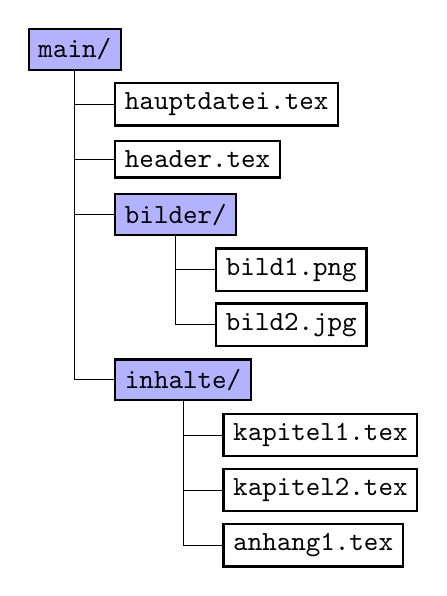
\begin{tikzpicture}[
	every node/.style={draw=black,thick,anchor=west},
	grow via three points={one child at (0.5,-0.7) and two children at (0.5,-0.7) and (0.5,-1.4)},
 	edge from parent path={(\tikzparentnode.south) |- (\tikzchildnode.west)}]
 	\ttfamily
	\node [fill=blue!30] {main/}
		child {node {hauptdatei.tex}}
		child {node {header.tex}}
%		child {node {defs}}
		child {node [fill=blue!30] {bilder/}
			child {node {bild1.png}}
			child {node {bild2.jpg}}
		}
		child [missing] {}
		child [missing] {}
		child {node [fill=blue!30] {inhalte/}
			child {node {kapitel1.tex}}
			child {node {kapitel2.tex}}
			child {node {anhang1.tex}}
		}
	;
\end{tikzpicture}
\end{column}
\end{columns}
\end{frame}
\MakeShortVerb|

\begin{frame}[fragile]{input \& include}
	\begin{itemize}
		\item \verb|\input| und \verb|\include| fügen externe Dateien am angegebenen Ort ein
		\item \TeX\ „springt“ aus dem aktuellen Dokument, liest woanders, und springt wieder zurück \pause
		\item \TeX-Version: \verb|\input| liest den Code einfach ein, als gehöre er ins Hauptdokument
		\item \LaTeX-Version: |\include| erstellt eigene \verb|.aux|-Datei (sinnvoll, wenn \verb|.aux| benötigt)
		\item \verb|\includeonly{a.tex,b.tex}| in der Präambel lässt nur die angegebenen Dateien für \verb|\include| zu
		\item \verb|\excludeonly{b.tex,c.tex}| lässt die angegebenen Dateien für \verb|\include| \emph{nicht} zu (benötigt Paket \pkg{excludeonly})
	\end{itemize}
\end{frame}

\begin{frame}[fragile]{root-Dokument}
\begin{itemize}
	\item nach Aufteilung muss immer das Hauptdokument kompiliert werden
	\item[⇒] ständiges Wechseln zwischen Dokumenten\pause
	\item gute Editoren nehmen die Arbeit ab:
	\begin{itemize}
		\item Definition von Hauptdokumenten möglich
		\item Kompiliert automatisch das zugehörige Hauptdokument
	\end{itemize}
\end{itemize}
\pause\vfill
\begin{description}
\item[\parbox{2cm}{\vspace{-5.68cm}\flushright\TeX works\\\TeX shop\\\TeX studio}] 
Setzen von \emph{magic comments:}\\ \verb*?% !TEX root = ?\meta{Hauptdokument}
\begin{lstlisting}
% !TEX root = ../Masterarbeit.tex
% !TEX program = lualatex
% !TEX encoding = utf8
% !TEX spellcheck = de_DE
\end{lstlisting}
\item[Overleaf] Menu\,→\,Main Document
\item[viele IDEs] Festlegen einer „Projekt-Hauptdatei“
\end{description}
\end{frame}

\begin{frame}[fragile,t]{Beispiel-Hauptdokument}
\begin{lstlisting}
\input{header}

\includeonly{chapter1}
\excludeonly{anhang} % erfordert Paket excludeonly!

\begin{document}
  \include{chapter1}
  \include{chapter2}
   ...
  \appendix
  \include{anhang}
\end{document}
\end{lstlisting}
\vfill
⇒ Nur \verb|chapter1| wird hier gesetzt, \verb|anhang| explizit nie.
\overleaf{tex20}
\end{frame}

\begin{frame}[fragile]{Header-Dokument}{Einstellungen}
	\begin{itemize}
		\item Satzspiegel
		\item Schriften (Brotschrift, Überschriften)
		\item Formatierung von Formeln
		\item …
		\item alles, was vor \verb|\begin{document}| steht
	\end{itemize}
\end{frame}

\begin{frame}[fragile,t]{Titelei}
	\begin{itemize}
		\item enthält alles bis zur ersten Inhaltsseite
		\item enthält Autor, Titel, etc.
		\item mit KOMA: Dokumentoption \verb|titlepage=true/false| setzt eigene Seiten oder einen Titelkopf
		\item Umgebung \verb|\begin{titlepage}| setzt eine frei gestaltbare Titelseite
		\item Befehl \verb|\maketitle| setzt vordefinierte Titelei
		\item Angaben von \verb|\title|, \verb|\author|, \verb|\extratitle| etc. nötig und möglich
	\end{itemize}
	\overleaf{tex14}
\end{frame}

\begin{frame}[fragile,t]{Titeleibefehle im KOMA-Bundle}
\begin{lstlisting}
\documentclass{scrbook}
\begin{document}
  \titlehead{\Large Universität Schlauenheim}
  \subject{Masterarbeit}
  \title{Risikomanagement in Zeiten von Social Media}
  \subtitle{Design interaktiver Apps für Banken und
    Versicherungen}
  \author{cand.\,stup. Uli Ungenau}
  \date{30. Februar 2017}
  \publishers{Betreut durch Prof.\,Dr.\,rer.\,stup. Naseweis}
  \dedication{Für meine Mama.}

  \maketitle
\end{document}
\end{lstlisting}
\end{frame}

\begin{frame}[fragile,b]{|\textbackslash maketitle| (in der Beamer-Klasse)}
\begin{LTXexample}[pos=b]
\title{Risikomanagement in Zeiten von Social Media}
\subtitle{Design interaktiver Apps für Banken und
  Versicherungen}
\author{cand.\,stup. Uli Ungenau}
\date{30. Februar 2017}

\maketitle
\end{LTXexample}
\end{frame}

\begin{frame}[fragile,t]{abstract}
\begin{itemize}
	\item Umgebung \verb|abstract| existiert für eine kurze Zusammenfassung des Dokuments
	\item mehrere Abstracts möglich (z.\,B. englisch\,/\,deutsch etc.)
\end{itemize}
\vfill
\begin{LTXexample}
\begin{abstract}
  Hier kommt eine kurze Zusammenfassung des Inhalts \dots
\end{abstract}

Und hier fängt das eigentlich Dokument an 
\dots
\end{LTXexample}
Die \texttt{abstract}-Umgebung steht in der \texttt{scrbook}/\texttt{book}-Klasse nicht zur Verfügung.
\end{frame}

\begin{frame}[fragile]{Verzeichnisse – TOC, LOF, LOT}
	\begin{itemize}
		\item Verzeichnisse fassen strukturierte Elemente zusammen
		\item prinzipiell kann alles in ein eigenes Verzeichnis aufgenommen werden
		\item übliche Verzeichnisse:
		\begin{itemize}
			\item Inhaltsverzeichnis \hfill \verb|\tableofcontents|
			\item Abbildungsverzeichnis \hfill \verb|\listoffigures|
			\item Tabellenverzeichnis \hfill \verb|\listoftables|
		\end{itemize}
		\item Aufnamhme der Verzeichnisse ins Inhaltsverzeichnis:
		 |\setuptoc{toc}{totoc}|
%		\item möglich: Codeverzeichnis, Beispielverzeichnis, …
	\end{itemize} 
\end{frame}

\begin{frame}[fragile]{Fußnoten, Randbemerkungen}
	zusätzlicher Text, der nicht ins Hauptdokument\,/\,in den Textfluss passt
	\begin{itemize}
		\item Fußnoten \hfill \verb|\footnote{}|
		\item gleitende Randnotiz \hfill \verb|\marginpar|
		\item Randbemerkung  (Paket \pkg{marginnote}) \hfill \verb|\marginnote|
	\end{itemize}
	\vfill
	Paket \pkg{footmisc} bietet vielfältige Möglichkeiten Aussehen von Fußnoten anzupassen
\end{frame}

\begin{frame}[fragile]{Zitate}
Es gibt eigene Umgebungen für Zitate:
\begin{itemize}
\item \verb|quote| für kurze Zitate
\item	 \verb|quotation| für längere Zitate
\item \verb|verse| für Gedichte
\end{itemize}
Das Paket \pkg{csquotes} passt Feinheiten von Anführungszeichen für den nicht-englischen Satz an.
\vfill
\begin{lstlisting}
\begin{quote}
  alea iacta est \hfill\textit{Caesar}
\end{quote}
\end{lstlisting}
\end{frame}

\begin{frame}[fragile]{Verweise}
	\begin{itemize}
		\item Elemente können mittels \verb|\label{}| bezeichnet werden
		\item mögliche Elemente sind Überschriften (sections etc.), \verb|table|, \verb|figure|, Formeln, …
		\item Referenzierung mit \verb|\ref{}| oder \verb|\cref| (Paket \pkg{cleveref})
	\end{itemize}
\end{frame}

\begin{frame}[fragile,t]{Links im Dokument}{hyperref}
\begin{itemize}
\item Paket \pkg{hyperref} macht Verweise im PDF anklickbar
\item \verb|\ref| und \verb|\cite| wird automatisch verlinkt
\item	 URLs können mit \verb|\url{|\meta{URL}\verb|}| angegeben werden
\item	 benannte Links mit \verb|\href{|\meta{URL}\verb|}{|\meta{angezeigter Text}\verb|}|
\end{itemize}
\uncover<2>{Um Probleme zu vermeiden \pkg{hyperref} eher als letztes Paket laden!}
\vfill
\begin{LTXexample}
\url{http://xkcd.com}\\
\href{mailto:mail@latexkurs.de}{\huge\Letter}
\end{LTXexample}
\end{frame}

\begin{frame}[fragile]{Vorspann\,/\,Anhang in \texttt{scrbook}}
\begin{itemize}
\item Befehl |\frontmatter| schaltet auf römische Seitenzahlen
\item |\mainmatter| auf normaler Nummerierung 
\item |\backmatter| auf Anhang \\ in anderen Dokumentenklassen:  nur |\appendix|
\item Nummerierung startet neu\\(abhängig von Dokumentenklasse A, B, C, …)
\item Abschnitte im Anhang wie gewohnt mit |\chapter|, |\section|, etc.
\end{itemize}
\vfill
\begin{lstlisting}
\frontmatter
\mainmatter
\backmatter
\end{lstlisting}
\end{frame}


\begin{frame}{Anwendung}
\begin{arbeitsauftrag}
Ergänzen Sie Ihr Dokument um die folgenden Elemente:
\begin{itemize}
\item Titelseite
\item Inhaltsverzeichnis
\item Abbildungsverzeichnis
\item Tabellenverzeichnis
\item Anhang
\end{itemize}
\end{arbeitsauftrag}
\end{frame}


%%%%%%%%%%%%%%%%%%%%%%%%%%%%%%%%%%%%%%%%%%%%%%%%%%%%%%%%%%%%%%%%%%%%%%%%%%%%%%%%%%%%%%%%%%%%%%%%%%%%%%%%%%
\teil{Diagramme}
%%%%%%%%%%%%%%%%%%%%%%%%%%%%%%%%%%%%%%%%%%%%%%%%%%%%%%%%%%%%%%%%%%%%%%%%%%%%%%%%%%%%%%%%%%%%%%%%%%%%%%%%%%

\begin{frame}{Diagramme}
\begin{itemize}
\item Ein Diagramm ist eine grafische Darstellung von Daten, Sachverhalten oder Informationen.
\item Information sollte dabei im Vordergrund stehen
\item Diagramme sollten sich in das Dokument einfügen
\begin{itemize}
\item passende Dimensionen
\item Beschriftung in gleicher Schriftart
\end{itemize}
\end{itemize}

Empfehlung für Diagramme in \LaTeX: \pkg{pgfplots}
\end{frame}

\begin{frame}[fragile]{pgfplots}
Konfiguration mittels \verb|\pgfplotsset{|\meta{Optionen}|}|. Paketautor empfiehlt, für zukünftige Kompatbilität, die aktelle Version anzugeben.
\begin{lstlisting}
\usepackage{pgfplots}
\pgfplotsset{compat=1.17}
\end{lstlisting}
\pause
\pkg{pgfplots} basiert auf \href{http://ctan.org/pkg/pgf}{\TikZ/PGF} und steht deshalb innerhalb einer |tikzpicture|:
\begingroup
\pgfplotsset{scale=0.5}
\begin{LTXexample}[pos=r, explpreset={}, preset=, rframe={}]
\begin{tikzpicture}
  \begin{axis}
    ...
  \end{axis}
\end{tikzpicture}
\end{LTXexample}
\endgroup
\overleaf{tex15}
\end{frame}


\begin{frame}{Achsentypen}
Verschiedene Achsentypen verfügbar: \\[1em]
\texttt{\textbackslash begin\{}\meta{Achsentyp}\verb|\}[|\meta{Optionen}\verb|]|\\
\quad\meta{Inhalt}\\
\texttt{\textbackslash end\{}\meta{Achsentyp}\verb|\}|

\vfill

\begin{tabular}{rl}
\verb|axis| & lineare Koordinatenachsen\\
\verb|semilogyaxis| & $x$-Achse linear, $y$-Achse logarithmisch\\
\verb|semilogxaxis| & $x$-Achse logarithmisch, $y$-Achse linear\\
\verb|loglogaxis| & beide Achsen logarithmisch\\
\verb|polaraxis| & Polarkoordinaten\footnote{mit \verb|\textbackslash usepgfplotslibrary\{polar\}|}\\
\verb|smithchart| & Smith-Diagramm\footnote{mit \verb|\textbackslash usepgfplotslibrary\{smithchart\}|}\\
\verb|ternaryaxis| & Dreiecksdiagramm\footnote{mit \verb|\textbackslash usepgfplotslibrary\{ternary\}|}
\end{tabular}
\end{frame}


\begin{frame}[fragile,t]{Daten hinzufügen}%\verb|\textbackslash addplot|}
\verb|\addplot [|\meta{Optionen}\verb|] {|\meta{Eingabedaten}\verb|};|\\%\meta{ggf. TikZ-Befehle}|;|\\
\verb|\addplot+[|\meta{Optionen}\verb|] {|\meta{Eingabedaten}\verb|};|%\meta{ggf. TikZ-Befehle}|;|
\pdfmarginpar{Während die angegebenen Optionen bei addplot die globalen/bzw. Standardoptionen überschreiben fügt addplot+ die angegebenen Optionen nur den globalen hinzu.}\vfill
\begin{LTXexample}[pos=r, explpreset={}, preset=\small, rframe={}]
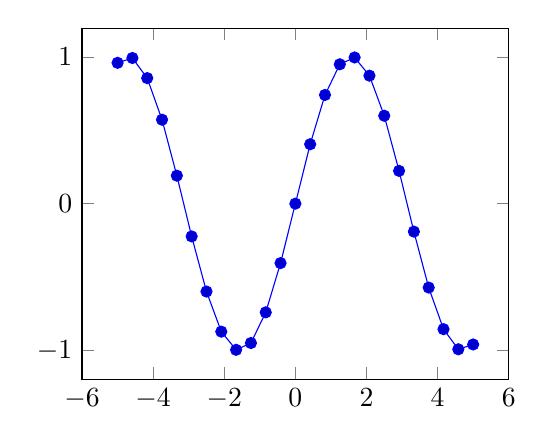
\begin{tikzpicture}
  \begin{axis}
    \addplot{sin deg(x)};
  \end{axis}
\end{tikzpicture}
\end{LTXexample}
\end{frame}

\begin{frame}[fragile,t]{Koordinaten Eingabe}
\verb|\addplot [|\meta{Optionen}\verb|] coordinates {|\meta{Koordinaten}\verb|};|\vfill
\begin{LTXexample}[pos=r, explpreset={}, preset=\small, rframe={}]
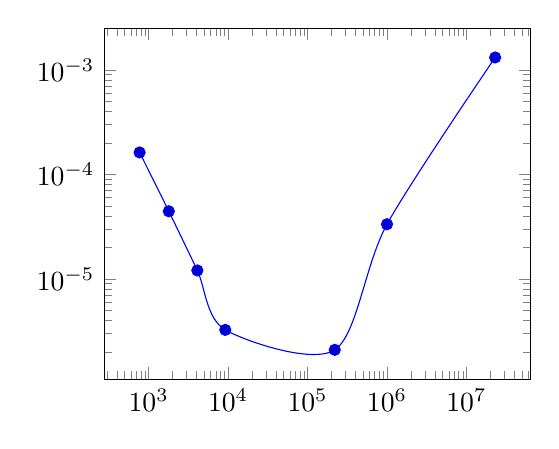
\begin{tikzpicture}
  \begin{loglogaxis}
    \addplot+[smooth]
     coordinates {
      (769, 1.6227e-04)
      (1793, 4.4425e-05)
      (4097, 1.2071e-05)
      (9217, 3.2610e-06)
      (2.2e5, 2.1E-6)
      (1e6, 0.00003341)
      (2.3e7, 0.00131415)
    };
  \end{loglogaxis}
\end{tikzpicture}
\end{LTXexample}
\end{frame}


\begin{frame}[fragile,t]{Daten-Tabellen}
\verb|\addplot [|\meta{Optionen}\verb|] table [|\meta{Spalten-Auswahl}\verb|] {|\meta{Tabelle}\verb|};|\pdfmarginpar{Tabelle kann dabei entweder eine Datei mit Tabellendaten, oder eine direkt im TeX-File eingegebe Tabelle sein.}
\vfill
\begin{LTXexample}[pos=r, explpreset={}, preset=\small, rframe={}]
\begin{tikzpicture}
  \begin{axis}
    \addplot table [
      only marks,
    ] {
      x    y    myvalue 
      0.5  0.2  0.25
      0.2  0.1  1.5
      0.7  0.6  0.75
      0.35 0.4  0.125
      0.65 0.1  2
    };
  \end{axis}
\end{tikzpicture}
\end{LTXexample}
\end{frame}


\begin{frame}[fragile,t]{Daten in externen Dateien}
\verb|\addplot [|\meta{Optionen}\verb|] table [|\meta{Spalten-Ausw.}\verb|] {|\meta{Dateipfad}\verb|};|\vfill
\begin{LTXexample}[pos=r, explpreset={}, preset=\small, rframe={}]
\begin{tikzpicture}
  \begin{axis}
    \addplot [no markers]
      table
      [x=time, y=values]
      {data.dat};
  \end{axis}
\end{tikzpicture}
\end{LTXexample}
\pause
Paket \pkg{pgfplotstable} erlaubt das Nachbearbeiten vorhandener Tabellen (z.\,B. Einfügen einer Ausgleichsgerade).
\end{frame}

\begin{frame}[fragile]{Beschriftungen}
\begin{tabular}{rll}
Key & Values & Funktion\\\midrule
\verb|title| & Text & Titel über dem Diagramm\\
\verb|x|/\verb|ylabel| & bel. Text & Beschriftung der $x$- bzw. $y$-Achse  \\
\verb|x|/\verb|ymin|/\verb|max| & Wert & schränkt Achse auf Bereich ein\\
\verb|mark| & \verb|*|, \verb|x|, \verb|+|, \verb|o|, … & Koordinaten-Marker anpassen\\
\verb|x|/\verb|ytick| & Liste & Koordinatenstriche explizit angeben\\
\verb|minor tick num| & Zahl & Anzahl der Zwischenstriche\\
\verb|grid| & \verb|major|, \verb|minor| & Gitter im Hintergrund einblenden
\end{tabular}
\end{frame}

\begin{frame}[fragile,t]{Lengenden}
\verb|\addlegendentry{|\meta{Beschreibung}\verb|}|\vfill
\begin{LTXexample}[pos=r, explpreset={}, preset=\small, rframe={}]
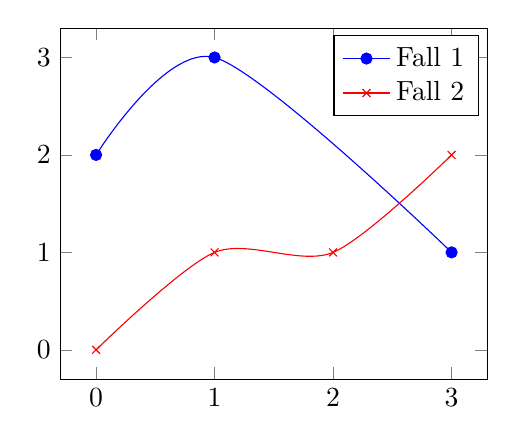
\begin{tikzpicture}
\begin{axis}
  \addplot[smooth,mark=*,blue] coordinates {
    (0,2) (1,3) (3,1)
  };
  \addlegendentry{Fall 1}
  \addplot[smooth,color=red,mark=x] coordinates {
    (0,0) (1,1) (2,1) (3,2)
  };
  \addlegendentry{Fall 2}
\end{axis}
\end{tikzpicture}
\end{LTXexample}
\end{frame}

\begin{frame}[fragile,t]{Platzierung der Achsen}
\verb|axis y line=|\meta{Platzierung}, \verb|axis x line=|\meta{Platzierung}\vfill
\begin{LTXexample}[pos=r, explpreset={}, preset=\small, rframe={}]
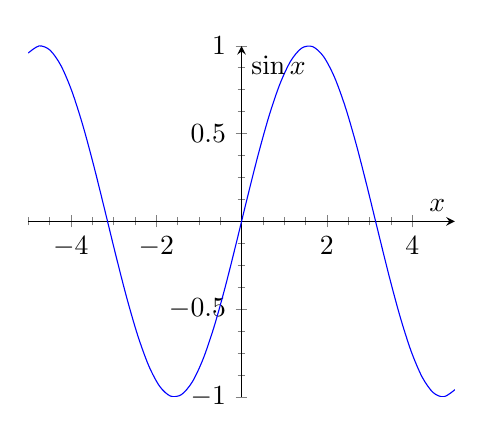
\begin{tikzpicture}
\begin{axis}[
minor tick num=3,
axis y line=center,
axis x line=middle,
xlabel=$x$,ylabel=$\sin x$
]
\addplot[smooth,blue,mark=none,
domain=-5:5,samples=40]
{sin(deg(x))};
\end{axis}
\end{tikzpicture}
\end{LTXexample}
\end{frame}

\begin{frame}[fragile,t]{Fehlerbalken}
Fehler können mit den Optionen \verb|error bars/|\meta{Key}\verb|=|\meta{Value} gesetzt werden.\vfill
\begin{LTXexample}[pos=r, explpreset={}, preset=\small, rframe={}]
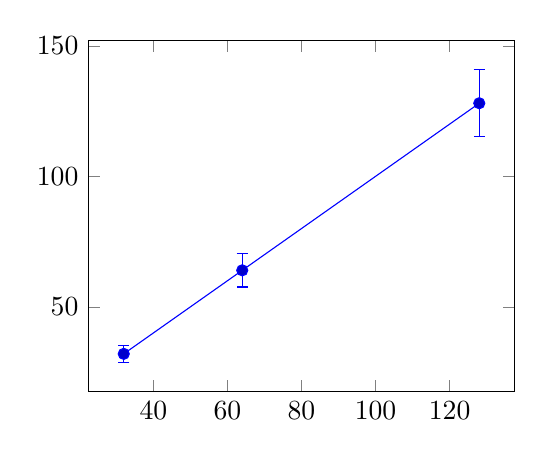
\begin{tikzpicture}
\begin{axis}
  \addplot+[
   error bars/y dir=both,
   error bars/y fixed relative=.1,
  ] table [x=x,y=y]
  {x	    y
   32     32
   64     64
   128    128
  };
\end{axis}
\end{tikzpicture}
\end{LTXexample}
\end{frame}

\begin{frame}[fragile,t]{Fehlerbalken}
Individuelle Fehler konnen mit \verb|+-| (symmetrisch) oder \verb|+=| und \verb|-=| (asymmetrisch) angegeben werden:\vfill
\begin{LTXexample}[pos=r, explpreset={}, preset=\small, rframe={}]
\begin{tikzpicture}
\begin{axis}
  \addplot+[
    error bars/.cd,
    x dir=both,
    x explicit,
    y dir=both, 
    y explicit,
  ] coordinates {
    (1,1) += (0.4,0.2) 
          -= (0.1,0.1)
    (3,2) -= (1,0)
    (4,5) +- (0.3,0.2)
  };
\end{axis}
\end{tikzpicture}
\end{LTXexample}
\end{frame}

\begin{frame}[fragile,t]{Fehlerbalken}
Fehler können auch aus einer Tabelle stammen:\vfill
\begin{LTXexample}[pos=r, explpreset={}, preset=\small, rframe={}]
\begin{tikzpicture}
  \begin{axis}
    \addplot [only marks, mark=x, 
    error bars/.cd,
    y dir=both, y explicit,]
      table
      [x=time, y=values, y error=error]
      {data.dat};
  \end{axis}
\end{tikzpicture}
\end{LTXexample}
\end{frame}


\begin{frame}[fragile,t]{Histogramme}
Histogramme mit Option \verb|hist={|\meta{Histogram-Optionen}\verb|}|\vfill
\begin{LTXexample}[pos=r, explpreset={}, preset=\small, rframe={}]
\begin{tikzpicture}
  \begin{axis}
    \addplot+[
      fill=blue!40!white,
      mark={},
      hist={
        data=y, 
        bins=10
      }
    ] table {data.dat};
  \end{axis}
\end{tikzpicture}
\end{LTXexample}
Interessante Optionen:\\\verb|cummulative| für kummuliertes Histogram\\\verb|density| normiert auf 1
\end{frame}


\begin{frame}[fragile,t]{Balkendiagramme}
Option \verb|xbar| erzeug Balkendiagramm, \verb|ybar| erzeugt Säulendiagramm\vfill
\begin{LTXexample}[pos=r, explpreset={}, preset=\small, rframe={}]
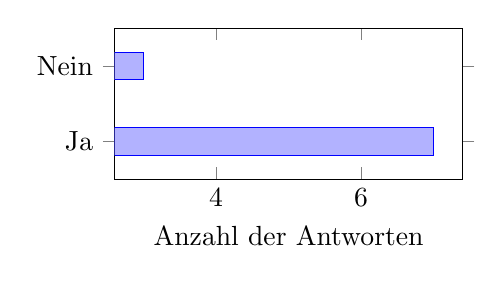
\begin{tikzpicture}
\begin{axis}[
 xbar,
 width=6cm, height=3.5cm,
 enlarge y limits=0.5,
 xlabel={Anzahl der Antworten},
 symbolic y coords={Ja,Nein},
 ytick=data,
]
 \addplot coordinates
  {(3,Nein) (7,Ja)};
\end{axis}
\end{tikzpicture}
\end{LTXexample}
\end{frame}


\begin{frame}[fragile,t]{Balkendiagramme}
Option \verb|xbar| erzeug Balkendiagramm, \verb|ybar| erzeugt Säulendiagramm\vfill
\begin{LTXexample}[pos=r, explpreset={}, preset=\small, rframe={}]
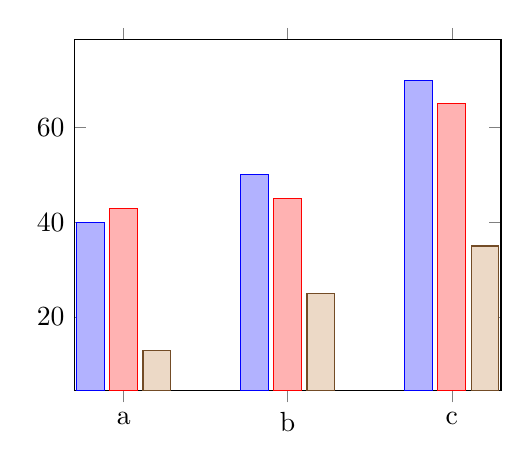
\begin{tikzpicture}
\begin{axis}[
 ybar,enlargelimits=0.15,
 symbolic x coords={a,b,c},xtick={a,b,c},
]
 \addplot coordinates 
 {(a,40) (b,50) (c,70)};
 \addplot coordinates 
 {(a,43) (b,45) (c,65)};
 \addplot coordinates 
 {(a,13) (b,25) (c,35)};
\end{axis}
\end{tikzpicture}
\end{LTXexample}
\end{frame}



\begin{frame}[fragile,t]{Boxplots}
\verb|\usepgfplotslibrary{statistics}| erlaubt Satz von Boxplots:\vfill
\usepgfplotslibrary{statistics}
\begin{LTXexample}[pos=r, explpreset={}, preset=\small, rframe={}]
\begin{tikzpicture}
  \begin{axis}
    \addplot+[
    boxplot prepared={
      median=4000,
      upper quartile=5500,
      lower quartile=3000,
      upper whisker=1200,
      lower whisker=15000,
    } ] coordinates {};
  \end{axis}
\end{tikzpicture}
\end{LTXexample}
\end{frame}

\begin{frame}[fragile,t]{3D-Plots}% \verb|\textbackslash addplot3|}
\verb|\addplot3 [|\meta{Optionen}\verb|] {|\meta{Eingabedaten}\verb|};| \vfill
\begin{LTXexample}[pos=r, explpreset={}, preset=\small, rframe={}]
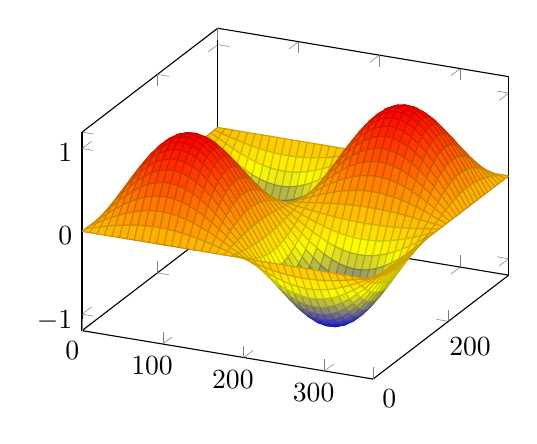
\begin{tikzpicture}
  \begin{axis}
    \addplot3[
      surf,
      domain=0:360,
      samples=40,
    ]
    {sin(x)*sin(y)};
  \end{axis}
\end{tikzpicture}
\end{LTXexample}
\end{frame}

%% TikZ-Diagramme aus R exportieren: R-Paket “TikZDevice”


\nocite{mathmode, dante:mathe, amsmath, booktabs, dante:tabellen, dante:koma, pgfplots}
\begin{frame}[allowframebreaks]{Weiterführende Literatur}
\printbibliography
\end{frame}


\begin{frame}<handout:0>{Lehrevaluation}

\begin{columns}
	\column{.4\textwidth}
	\href{https://evasys.uni-mannheim.de/evasys/online.php?p=\kursAB{\evallosungA}{\evallosungB}}{\qrcode[height=\textwidth]{https://evasys.uni-mannheim.de/evasys/online.php?p=\kursAB{\evallosungA}{\evallosungB}}}
	\column{.55\textwidth}
	\begin{tabbing}
	\textbf{Losung:\quad}\=\url{evasys.uni-mannheim.de} \kill
	\textbf{Link:} \> \href{https://evasys.uni-mannheim.de/evasys/online.php?p=\kursAB{\evallosungA}{\evallosungB}}{\texttt{evasys.uni-mannheim.de}} \\
	\textbf{Losung:} \> \href{https://evasys.uni-mannheim.de/evasys/online.php?p=\kursAB{\evallosungA}{\evallosungB}}{\texttt{\kursAB{\evallosungA}{\evallosungB}}}
	\end{tabbing}
\end{columns}
\end{frame}


\AtEndDocument{\frame{\centering \Huge Happy \TeX ing}}

\end{document}